\section{Método de Interpolação}

\begin{enumerate}

\item Transforma o polinômio característico em um polinômio de interpolação \textit{forward} de Newton.

\item Converte o polinômio \textit{forward} de Newton em uma série de potências.

\item Calcula as raízes da função pelo método de Bairstow.

\end{enumerate}

\begin{itemize}

\item Matriz de ordem $ N \Rightarrow $ polinômio característico de grau $ N $.

\item Se construirmos uma tabela $ \lambda \times f(\lambda) $ para $ n + 1 $ valores uniformemente espaçados de $ \lambda $, então $ f(\lambda) $ pode ser expresso por um polinômio de interpolação \textit{forward} de Newton.

\[
 f(\lambda) = g(s) = \sum_{n=0}^N \, \left(s \atop n\right) \, \Delta^n \, f_0
\]

com

\[
 f_i = f(\lambda_i), \, \, i = 0, 1, 2, \ldots, N
\]

\[
 s = \frac{\lambda - \lambda_0}{\Delta \, \lambda}
\]

\[
 \lambda_i = \lambda_{i-1} + \Delta \, \lambda
\]


\begin{itemize}

\item Como são calculados os $ f_i $'s ?

\[
 f_i = f(\lambda_i) = det \, (A - \lambda_i \, I)
\]

\item Como escolhemos $ \lambda_0 $ e $ \lambda_N $ ?

\textit{Teorema de Gerschgorin} (discos de \textit{Gerschgorin})

Considere que os autovetores estão normalizados de forma que o maior elemento fique igual a $ 1 $. Assim, se o maior elemento do autovetor $ q $ é o k-ésimo,

\[
 \lambda - a_{kk} = \sum_{j \neq k} \, a_{kj} \, q_j
\]

como

\[
 | \, q_j \, | \leq 1 \Rightarrow | \, \lambda - a_{kk} \, | \leq \displaystyle \sum_{j \neq k} \, | \, a_{kj} \, |
\]

Antes de calcularmos os autovetores, não podemos saber qual a linha $ k $ do termo máximo. Assim, os autovalores $ \lambda $ estão na união dos discos centrados em cada um dos termos $ a_{kk} $ da matriz $ A $ com raio igual a

\[
 \sum_{j \neq k} | \, a_{kj} \, |
\]

Por exemplo, o determinante de $ \lambda_0 $ e $ \lambda_N $ para a matriz

\[
 \left[
  \begin{array}{rrr}
   3 & 1 & 5\\
   1 & 3 & 5\\
   5 & 5 & -1
  \end{array}
 \right]
  \begin{array}{ll}
   \rightarrow & r = 1 + 5 = 6\\
   \rightarrow & r = 1 + 5 = 6\\
   \rightarrow & r = 5 + 5 = 10
  \end{array}
\]

\begin{figure}[htb]
 \centering
 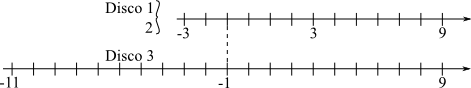
\includegraphics[scale=0.8]{capitulos/capitulo5/figuras/met_inter1.png}
 \caption{?}
 \label{fig:met_inter1}
\end{figure}

\begin{center}
 \framebox{ $ \lambda_0 = -11 $ } \, e \, \framebox{ $ \lambda_N = 9 $ }
\end{center}

\item Como transformar \, $ g(s) = \displaystyle \sum_{n=0}^N \, \left(s \atop n\right) \, \Delta^n \, f_0 $ \, em \, $ g(s) = f_0 + \displaystyle \sum_{i=1}^N \, b_i \, s $

\[
 \left(s \atop n\right) = \frac{s \, (s-1) \, (s-2) \ldots (s-n+1)}{n!} = \sum_{i=1}^n \, c_{n,i} \, s^i \, \, \, \, \, \, \, \, n \geq 1
\]

\[
 \begin{array}{ll}
  g(s) & = f_0 + \displaystyle \sum_{n=1}^N \, \sum_{i=1}^n \, c_{n,i} \, s^i \, \Delta^n \, f_0 = f_0 + \sum_{i=1}^N \, \left( \sum_{n=1}^N \, c_{n,i} \, \Delta^n \, f_0 \right) \, s^i\\
       & = f_0 + \displaystyle \sum_{i=1}^N \, b_i \, s^i
 \end{array}
\]

onde

\[
 b_i = \sum_{n=i}^N \, c_{n,i} \, \Delta^n \, f_0
\]

\[
 c_{n,i} = \frac{(-1)^{n+i}}{n} \, \left[ \sum_{k=1}^{ \frac{(n-1)!}{(i-1)! \, (n-i)!} } \, \frac{1}{\alpha_k} \right]
\]

onde $ \alpha_k $ são as combinações $ (i-1) $ a $ (i-1) $ dos $ (n-1) $ primeiros números naturais.

\item Coeficientes de Markov, $ c_{n,i} $

\begin{table}[htp]
%\footnotesize
	\centering
		\begin{tabular}{|r||r|r|r|r|r|r|}
		\hline		
		\textbf{$ n \setminus i $} & 1 & 2 & 3 & 4 & 5 & 6\\
		\hline \hline 
		1 & 1 & & & & &\\
		\hline 
		2 & $ -1/2 $ & $ 1/2 $ & & & &\\
		\hline 
		3 & $ 1/3 $ & $ -1/2 $ & $ 1/6 $ & & &\\
		\hline 
		4 & $ -1/4 $ & $ 11/24 $ & $ -1/4 $ & $ 0.04167 $ & &\\
		\hline 
		5 & $ 1/5 $ & $ -5/12 $ & $ 0.29167 $ & $ -0.08333 $ & $ 0.00833 $ &\\
		\hline 
		6 & $ -1/6 $ & $ 137/360 $ & $ -0.31250 $ & $ 0.11806 $ & $ -0.02083 $ & $ 0.0??39 $\\
		\hline
		\end{tabular}
	\caption{Coeficientes de Markov.}
	\label{cap5:sec2:tab1}
\end{table}

\[
 \sum_{n=1}^N \, \sum_{i=1}^n \, c_{n,i} \, s^i \, \Delta^n \, f_0
\]\\ \\

\begin{figure}[htb]
 \centering
 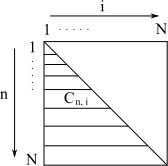
\includegraphics[scale=0.8]{capitulos/capitulo5/figuras/met_inter2.png}
 \caption{?}
 \label{fig:met_inter2}
\end{figure}

\[
 \sum_{i=1}^N \, \left( \sum_{n=i}^N \, c_{n,i} \, \Delta^n \, f_0 \right) \, s^i
\]

\[
 c_{6,5}
 = \frac{(-1)^{6+5}}{6} \, \left[ \sum_{k=1}^{\frac{(6-1)!}{(5-1)! \, (6-5)!}} \, \frac{1}{\alpha_k} \right]
 = \frac{-1}{6} \, \left[ \sum_{k=1}^{\frac{5!}{4! \, 1!}} \, \frac{1}{\alpha_k} \right]
 = \frac{-1}{6} \, \sum_{k=1}^5 \, \frac{1}{\alpha_k}
\]

\[
 \{1 \, 2 \, 3 \, 4 \, 5\} \equiv (n-1) \mbox{ primeiros números naturais}
\]

Combinações $ 4 $ a $ 4 $

\[
 \begin{array}{l}
  1 \, 2 \, 3 \, 4 \Rightarrow 1 \times 2 \times 3 \times 4 = 24 = \alpha_1\\
  1 \, 2 \, 3 \, 5 \Rightarrow 1 \times 2 \times 3 \times 5 = 30 = \alpha_2\\
  2 \, 3 \, 4 \, 5 \Rightarrow 2 \times 3 \times 4 \times 5 = 120 = \alpha_3\\
  1 \, 3 \, 4 \, 5 \Rightarrow 1 \times 3 \times 4 \times 5 = 60 = \alpha_4\\
  1 \, 2 \, 4 \, 5 \Rightarrow 1 \times 2 \times 4 \times 5 = 40 = \alpha_5
 \end{array}
\]

\[
 c_{6,5}
 = \frac{-1}{6} \, \left[ \frac{1}{24} + \frac{1}{30} + \frac{1}{40} + \frac{1}{60} + \frac{1}{120} \right]
 = - \frac{1}{48}
 = -0.02083
\]

\begin{example}

Encontre a série de potências da equação característica

\[
 f(\lambda)
 = det \,
 \left[
 \begin{array}{rrr}
  3-\lambda & 4          & -2\\
  3         & -1-\lambda & 1\\
  2         & 0          & 5-\lambda
 \end{array}
 \right]
\]

\textbf{Solução:} $ g(\lambda) = -71 + \lambda + 7 \, \lambda^2 - \lambda^3 $\\


\[
 \begin{array}{lll}
  & & (3-\lambda) \, (-1-\lambda) \, (5-\lambda) + 8 - (2) \, (-2) \, (-1-\lambda) - 12 \, (5-\lambda)\\
  & = & (-3 -2 \, \lambda + \lambda^2) \, (5 - \lambda) + 8 + 4 \, (-1 -\lambda) - 60 + 12 \, \lambda\\
  & = & -15 -10 \, \lambda + 5 \, \lambda^2 + 3 \, \lambda + 2 \, \lambda^2 - \lambda^3 + 8 - 4 -4 \, \lambda - 60 + 12 \, \lambda\\
  g(\lambda) & = & -71 + \lambda + 7 \, \lambda^2 - \lambda^3
 \end{array}
\]

\end{example}

\begin{figure}[htb]
 \centering
 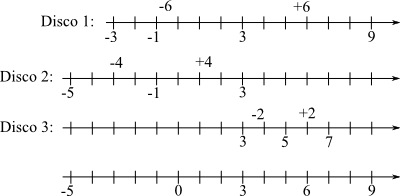
\includegraphics[scale=0.8]{capitulos/capitulo5/figuras/met_inter3.png}
 \caption{?}
 \label{fig:met_inter3}
\end{figure}

\[
\begin{array}{l}
 f(0) = det \,
 \left[
 \begin{array}{ccc}
  3 & 4 & -2\\
  3 & -1 & 1\\
  2 & 0 & 5
 \end{array}
 \right]
 = - 15 + 8 - 4 - 60 = -71\\
 f(3) = det \,
 \left[
 \begin{array}{ccc}
  0 & 4 & -2\\
  3 & -4 & 1\\
  2 & 0 & 2
 \end{array}
 \right]
 = 8 - 16 - 24 = -32\\
 f(6) = det \,
 \left[
 \begin{array}{ccc}
  -3 & 4 & -2\\
  3 & -7 & 1\\
  2 & 0 & -1
 \end{array}
 \right]
 = -21 + 8 - 28 + 12 = -29\\
 f(9) = det \,
 \left[
 \begin{array}{ccc}
  -6 & 4 & -2\\
  3 & -10 & 1\\
  2 & 0 & -4
 \end{array}
 \right]
 = -240 + 8 - 40 + 48 = -224
\end{array}
\]

\[
 g(s) = f(?) + b_1 \, s + b_2 \, s^2 + b_3 \, s^3
\]

\[
 \begin{array}{l}
  b_1 = c_{1,1} \, \Delta^1 \, f_0 + c_{2,1} \, \Delta^2 \, f_0 + c_{3,1} \, \Delta^3 \, f_0 = 1 \times (-32 + 71) - \frac{1}{2} (\\
  b_2 = c_{2,2} \, \Delta^2 \, f_0 + c_{3,2} \, \Delta^3 \, f_0\\
  b_3 = c_{3,3} \, \Delta^3 \, f_0
 \end{array}
\]

\end{itemize}

\end{itemize}

\begin{example}
 Testar os métodos de autovalores e autovetores considerando a matriz
simétrica M:

\[
M=\left[\begin{array}{ccc}
4 & 2 & 1\\
2 & 3 & 2\\
1 & 2 & 5\end{array}\right]\]


Achando a equacão característica do problema de autovalores e autovetores
associado à matriz M dada:

\[
f(\lambda)\equiv det\left[M-\lambda I\right]=0\]


\[
\left[\begin{array}{ccc}
4 & 2 & 1\\
2 & 3 & 2\\
1 & 2 & 5\end{array}\right]-\lambda\left[\begin{array}{ccc}
1 & 0 & 0\\
0 & 1 & 0\\
0 & 0 & 1\end{array}\right]=\left[\begin{array}{ccc}
4-\lambda & 2 & 1\\
2 & 3-\lambda & 2\\
1 & 2 & 5-\lambda\end{array}\right]\]


\[
det\left[\begin{array}{ccc}
4-\lambda & 2 & 1\\
2 & 3-\lambda & 2\\
1 & 2 & 5-\lambda\end{array}\right]=0\]


Logo:

\[
\lambda^{3}-12\lambda^{2}+38\lambda-29=0\]


\begin{center}
----------------------------------------------------------------------------------------------------------------------------------------------------
\par\end{center}

Sabendo que uma matriz simétrica com coeficientes reais tem apenas
autovalores reais, vamos utilizar o teorema dos discos de Gerschgorin
para determinar um intervalo no eixo dos números reais que contém
os autovalores de M. 

\[
M=\left[\begin{array}{ccc}
4 & 2 & 1\\
2 & 3 & 2\\
1 & 2 & 5\end{array}\right]\]


Os autovalores $\lambda$ estão na união dos discos centrados em cada
um dos termos $a_{kk}$ da matriz M com raio igual a:

\[
\sum_{j\neq k}|a_{kj}|\]


Ou seja, para $a_{11}$ temos:

\begin{center}
raio=$|a_{12}|+|a_{13}|=3$, centro em: (4,0)
\par\end{center}

Para $a_{22}$ temos:

\begin{center}
raio=$|a_{21}|+|a_{23}|=4$, centro em: (3,0)
\par\end{center}

Para $a{}_{33}$ temos:

\begin{center}
raio = $|a_{31}|+|a_{32}|=3$, centro em: (5,0)
\par\end{center}

Para definirmos o $\lambda_{0}$e o $\lambda_{n}$, basta pegarmos
o menor e o maior valor alcancado pelos circulos de Gerschgorin com
as características acima.

\[
\lambda_{0}=-1\]


\[
\lambda_{n}=8\]

\end{example}

\begin{example}
 Iremos calcular uma das raízes do polinômio característico, desenvolvido no exemplo anterior, pelo método de Newton-Raphson com precisão de 4 casas decimais. Deflacionaremos o polinômio característico e acharemos as outras raízes resolvendo o polinômio de segundo grau resultante do processo de deflação. 

Temos a seguinte equacao como equacao característica encontrada da matriz M:

\lambda^{3}-12\lambda^{2}+38\lambda-29=0

Usando o método e newton-raphson:

f(x)=\lambda^{3}-12\lambda^{2}+38\lambda-29

f^{'}(x)=3\lambda^{2}-24\lambda+38

\varepsilon=0,0001

Usaremos como estimativa inicial x_{0}=1, então teremos:

x_{1}=x_{0}-\frac{f(x)}{f^{'}(x)}

substituindo:

x_{1}=1-\frac{-2}{17}=1,117647059

testando critérios de parada, temos |f(x_{0})|=2 e |x_{1}-x_{0}|=0,1176, devemos continuar:

x_{2}=1,117647059-\frac{-0,122939138}{14,923875429}=1,125884808

testando critérios de parada, temos |f(x_{1})|=0,122939138 e |x_{2}-x_{1}|=0,008237749, devemos continuar:

x_{3}=1,125884808-\frac{-0,000586233}{14,781614411}=1,125923468

testando critérios de parada, temos |f(x_{2})|=0,000586233 e |x_{3}-x_{2}|=0,00003866, temos agora que |x_{3}-x_{2}|<\varepsilon, então devemos parar. Logo, temos como primeira raiz aproximada de f(x) o valor 1,125923468. Devemos agora achar as outras raízes.

Como temos que uma das raízes é aproximadamente 1,125923468 podemos usar a regra de Ruffini para deflacionar f(x) com o r sendo igual à raíz encontrada anteriormente. Teremos então,

\begin{array}{ccccccc}
\varnothing & | & +1 & -12 & +38 & | & -29\\
- & - & - & - & - & - & -\\
+1,125923468 & | & \varnothing & 1,125923468 & -12,24337796 & | & +28,999985211\\
- & - & - & - & - & - & -\\
\varnothing & | & +1 & -10,874076532 & +25,75662204 & | & -0,000014789\end{array}

Temos então a equacão: x^{2}+-10,874076532x+25,75662204 e como resto -0,000014789.

Tirando as outras raízes:

x^{2}+-10,874076532x+25,75662204=0

\Delta=(-10,874076532)^{2}-4*1*25,75662204=15,219052264

\sqrt{\Delta}=3,901160374

x=\frac{-(-10,874076532)\pm3,901160374}{2*1}

x_{1}=3,486458079

x_{2}=7,387618453

Logo, temos como raízes para a função f(x)=\lambda^{3}-12\lambda^{2}+38\lambda-29 os valores x_{1}=3,486458079, x_{2}=7,387618453 e x_{3}=1,125923468.

\end{example}

\begin{example}
Calcularemos os autovetores correspondentes aos autovalores encontrados no exemplo anterior, resolvendo os três sistemas de equações lineares homogêneos pelo método de eliminação de Gauss. 

Para encontrarmos os autovetores da matriz M em questão temos que encontrar o vetor de x que satisfaça a seguinte equação (7.1.5b página 259):\overline{M}x=0 onde \overline{M}=[M-\lambda] e x é um vetor da forma \begin{array}{c}
x_{1}\\
x_{2}\\
x_{3}\end{array}.

Temos então, teremos:

\left[\begin{array}{ccc}
(4-\lambda) & 2 & 1\\
2 & (3-\lambda) & 2\\
1 & 2 & (5-\lambda)\end{array}\right]*\left(\begin{array}{c}
x_{1}\\
x_{2}\\
x_{3}\end{array}\right)=\left(\begin{array}{c}
0\\
0\\
0\end{array}\right)

Iremos então usar eliminação de Gauss com o \lambda\approx1,1259, temos então:

\left[\begin{array}{ccc}
2,8741 & 2 & 1\\
2 & 1,8741 & 2\\
1 & 2 & 3,8741\end{array}\right]

No primeiro passo temos como pivô a{}_{11}=2,8741:

m_{21}=a_{21}/piv\hat{o}=2/2,8741=0,6958

m_{31}=a_{31}/piv\hat{o}=1/2,8741=0,3479

Teremos então que transformar a linha 2 usando a seguinte fórmula: L_{2}=L_{2}=m_{21}*L_{1}. E a linha 3 usando a fórmula: L{}_{3}=L_{3}-m_{31}*L_{1}. Teremos a matriz seguinte como resultado:

\left[\begin{array}{ccc}
2,8741 & 2 & 1\\
0 & 0,4825 & 1,3042\\
0 & 1,3041 & 3,5261\end{array}\right]

No segundo passo, escolhemos como pivô a{}_{22}=0,4825:

m_{32}=a_{32}/piv\hat{o}=1,3041/0,4825=2,7036

Teremos então que transformar a linha 3 da matriz usando a seguinte fórmula: L_{3}=L_{3}=m_{32}*L_{2}. Teremos a matriz seguinte como resultado:

M_{2}=\left[\begin{array}{ccc}
2,8741 & 2 & 1\\
0 & 0,4825 & 1,3042\\
0 & 0 & 0\end{array}\right]

Temos então que:

M_{2}*x=0

\left[\begin{array}{ccc}
2,8741 & 2 & 1\\
0 & 0,4825 & 1,3042\\
0 & 0 & 0\end{array}\right]*\left(\begin{array}{c}
x_{1}\\
x_{2}\\
x_{3}\end{array}\right)=\left(\begin{array}{c}
0\\
0\\
0\end{array}\right)

\begin{cases}
\begin{array}{c}
2,8741x_{1}+2x_{2}+x_{3}=0\\
0,4825x_{2}+1,3042x_{3}=0\end{array} & \begin{array}{c}
\end{array}\end{cases}

Teremos para escolhido x{}_{3}=1 que o auto-vetor é:

V=\left(\begin{array}{c}
1\\
-2,703\\
1,533\end{array}\right)
\end{example}



